\subsubsection{Diseño de los circuitos requeridos}

A partir de las ideas ya expresadas en los puntos anteriores, se comienza con el diseño del circuito principal del sistema. Este circuito lleva en su corazón la tarjeta ESP32, la cual será la encargada de comandar y de sincronizar todas las tareas. De igual forma, se considera como la distribución principal de la energía del sistema a los circuito con alimentación de 5V dc.

De esta forma, la placa principal, estará compuesta por la ESP32 y diversos headers que irán desde cada una de sus terminales a todos los demás módulos, por medio de cables dupont, que servirán para comunicar a todos los circuitos y sensores entre si.

En la figura \ref{fg:principal_esq} se puede ver como se pretende llevar la interconexión de cada uno de los módulos, simulando las entradas de la ESP32 y realizando las pistas en cada una de las puntas de salida a cada circuito externo, también se ve cómo sería la PCB para el funcionamiento del sistema (Figura \ref{fg:PCB_Principal})

\begin{figure}[h!]
            \centering
            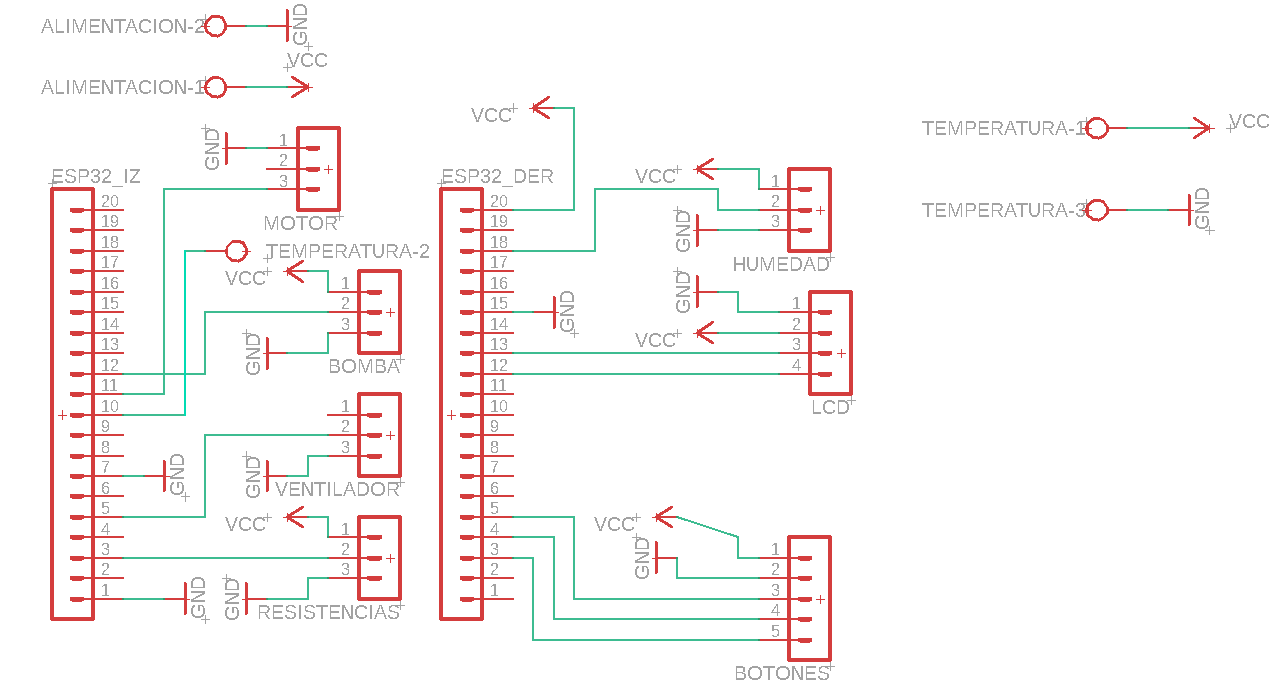
\includegraphics[scale=0.3]{images/Capitulo 4/3.1.1/principal.png}
            \caption{Circuito esquemático del cerebro del sistema}
            \label{fg:principal_esq}
        \end{figure}

\begin{figure}[h!]
            \centering
            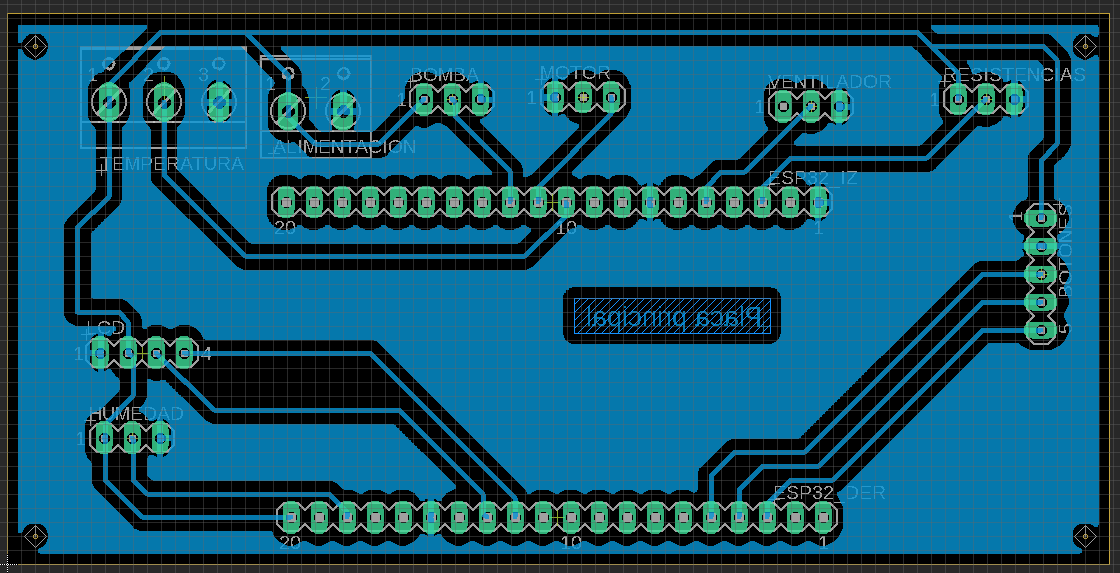
\includegraphics[scale=0.3]{images/Capitulo 4/3.1.1/Principal PCB.png}
            \caption{PCB principal del sistema}
            \label{fg:PCB_Principal}
        \end{figure}